\documentclass[10pt]{article}
\usepackage{graphicx}
\usepackage{xeCJK}
\usepackage{placeins}
\usepackage{float}
\usepackage{amsmath}

\setCJKmainfont{MS Mincho} % for \rmfamily
\setCJKsansfont{MS Gothic} % for \sffamily
\graphicspath{ {../image/} }
\renewcommand{\figurename}{図}
\renewcommand{\tablename}{表}

\title{Assignment 3}

\author{Phusaeng Natthaphat (04B23054)}
\date{2026年5月11日}


\begin{document}

\maketitle


\section{Set up}
\hspace*{\parindent} Consider the following damped osccilation.
\begin{align}
    m\dfrac{dv}{dt}&=-\zeta v- k x\label{eqn:v}\\
    v&=\dfrac{dx}{dt} \label{eqn:x}
\end{align}
by substitute (\ref{eqn:x}) in to (\ref{eqn:v}) we get second order ODE.
\begin{align}
    m\dfrac{d^2}{dt^2}x+\zeta\dfrac{dx}{dt}+kx=0
\end{align}
which has characteristic equation
\begin{align}
    m\lambda^2+\zeta\lambda+k=0
\end{align}
We can characterise behavior of the equation by different $\lambda$; Namely,
\begin{align}\label{eqn:case}
    \begin{cases}
        \zeta^2-4km>0&\text{overdamped}\\
        \zeta^2-4km<0&\text{underdamped}\\
        \zeta^2-4km=0&\text{critically damped}\\
    \end{cases}
\end{align}
Let's dedimensionalize (\ref{eqn:v}) by the following
\begin{align}
    \begin{split}
        x&=a\tilde{x}\\
        v&=\dfrac{a}{t_0}\tilde{v}\\
        t&=t_0\tilde{t}
    \end{split}
\end{align}
where $\tilde{x}, \tilde{v}, \tilde{t}$ are dimensionless.
\begin{align*}
    m\dfrac{a}{t_0}\dfrac{d\tilde{v}}{t_0d\tilde{t}}&=-\zeta\dfrac{a}{t_0}\tilde{v}-ka\tilde{x}\\
    0&=\dfrac{d\tilde{v}}{d\tilde{t}}+\dfrac{\zeta}{m}t_0\tilde{v}+\dfrac{k}{m}t_0^2\tilde{x}
\intertext{By substitute $t_d=m/\zeta$ and $t_s^2=m/k$ we get}
    0&=\dfrac{d\tilde{v}}{d\tilde{t}}+\dfrac{t_0}{t_d}\tilde{v}+\dfrac{t_0^2}{t_s^2}\tilde{x}
\end{align*}
Especially when choosing $t_0=t_s$ and define $\tau=t_s/t_d$ we get
\begin{align}
    0&=\dfrac{d}{d\tilde{t}}\tilde{v}+\tau\tilde{v}+\tilde{x}\\
    \tilde{v}&=\dfrac{d}{d\tilde{t}}\tilde{x}
\end{align}
with parameter $\tau>0$. Hence, we rewrite all possible outcomes in term of dimensionless parameter.
\begin{align}
    \begin{cases}
        \tau>2&\text{overdamped}\\
        \tau<2&\text{underdamped}\\
        \tau=2&\text{critically damped}\\
    \end{cases}
\end{align}
\section{Result}
With the following initial conditions
\begin{align}
    \begin{split}
        x(0)&=a\\
        v(0)&=0
    \end{split}
\intertext{or in dimensionless parameter}
    \begin{split}
        \tilde{x}(0)&=1\\
        \tilde{v}(0)&=0
    \end{split}
\end{align}
\begin{figure}[H]
    \centering
    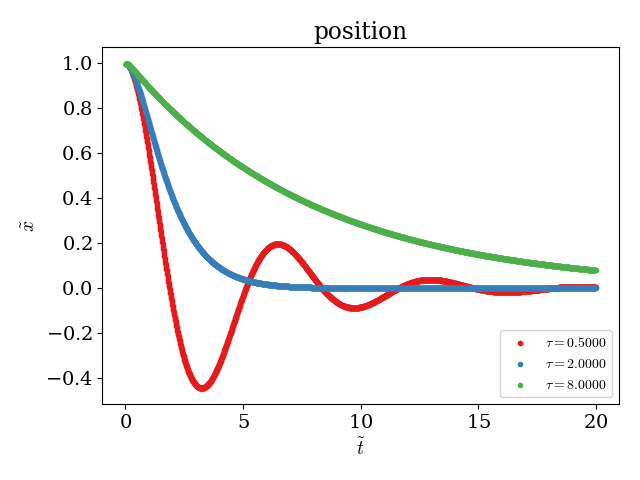
\includegraphics[width=\textwidth]{damped.png}
    \caption{Result}
\end{figure}
Clearly, the behavior of oscillation is dictated by dimensionless parameter $\tau$.

\end{document}